% Template for a Thesis
%
% 6-results.tex
%
% Results

\chapter{Results}\label{ch:results}

This chapter shows the results for each section of the development of this thesis, ranging from score plots for BPE alignments, to algorithm runtimes. The scores display four different metrics, which have been explained previously in the Translation chapter.~\ref{tra:metrics}

\section{Replication of BPE}

The results for BPE show that in the case of Fastalign, where the baseline F1 score is 0.6, and the best BPE result is with 1000 BPE merges, and a F1 score of 0.609.

\begin{figure}[!ht]
    \centering
    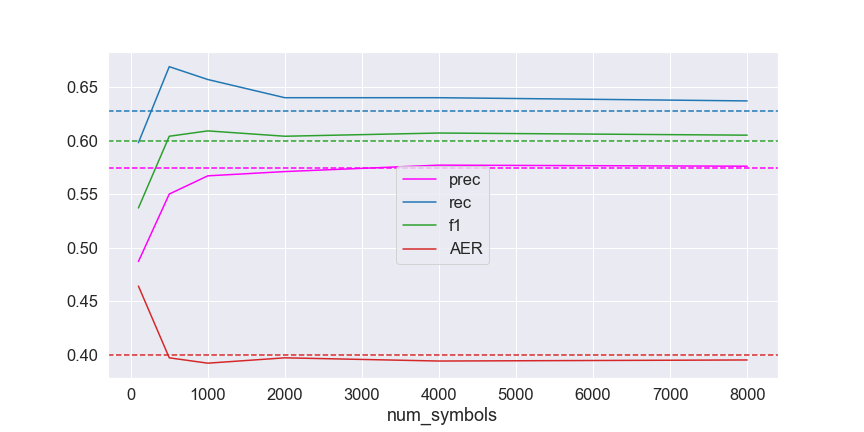
\includegraphics[width=12cm]{../reports/scores_normal_bpe/eng_deu_fastalign.png}
    \caption{Scores of BPE over baseline, using Fastalign}
\end{figure}

In the case of Eflomal, the baseline F1 score is 0.72, and the best BPE result is for 6000 BPE merges with a F1 score of 0.701. In absolute terms, BPE units using Eflomal have an absolute higher score than BPE units using Fastalign. But these values only make sense when compared against the baseline.

\begin{figure}[!ht]
    \centering
    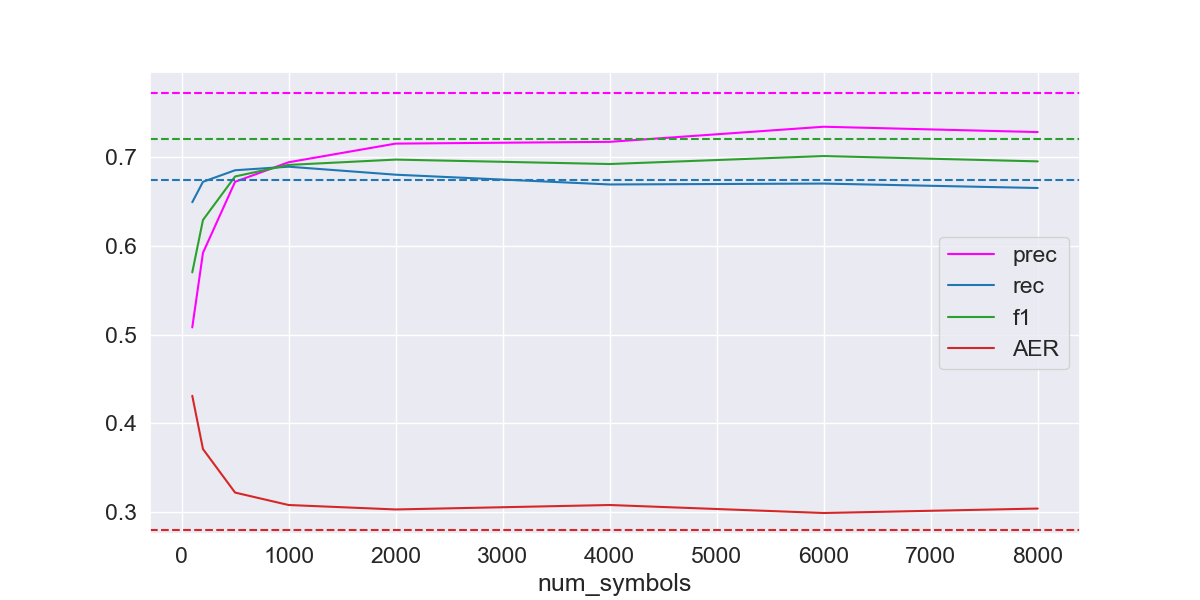
\includegraphics[width=12cm]{../reports/scores_normal_bpe/eng_deu_eflomal.png}
    \caption{Scores of BPE over baseline, using Eflomal}
\end{figure}

The alignment algorithms, Fastalign and Eflomal, require one language to be given as source and the other as target, and perform the alignment based on this. Throughout the thesis, English has been taken as the source language and German as the target. It might have been interesting to see that swapping the languages would yield different results, by swapping the languages in the global variables file. The difference between these two cases is barely perceptible, 0.03\% across all numbers of merges. Therefore, it is assumed that swapping the source and target language has no effect in the experiment result scores.

\section{Replication of BPE dropout}

When getting BPE dropout results, the desired comparison is that of BPE dropout with respect to BPE. As a result, the BPE scores are taken as baseline, instead of the gold standard scores as in the previous case. As explained in the Methodology chapter~\ref{met:replbpedrop}, the BPE dropout pipeline is run a number of times, resulting in many possible segmentations. Out of these, three types of results are obtained: union, intersection and threshold.

\begin{itemize}
	\item The \textbf{union} case takes all alignments into account, which results in a big list of alignments per sentence. These will most probably include the correct alignments, but there will many other wrong alignments. This case has low precision and high recall.
	\item The \textbf{intersection} case takes only those alignments which are present in all alignment files, resulting in a few number of alignments per sentence. Most probably, these alignments will be correct. But there will also be many alignment smissing. This case has high precision and low recall.
	\item The \textbf{threshold} case is a mixture between the previous two cases. Given a threshold, for instance 0.7, an alignemnt is accepted if it is present in 70\% of the alignment files. Smaller values for this variable resemble the union case, since more alignments are accepted. Higher threshold numbers resemble the intersection case, where alignments must be present in more and more files in order to be accepted.
\end{itemize}

The following figures show the results for a \emph{dropout} value of 0.1 or 10\%, and the union, intersection and threshold cases.

 \begin{figure}[!ht]
     \centering
     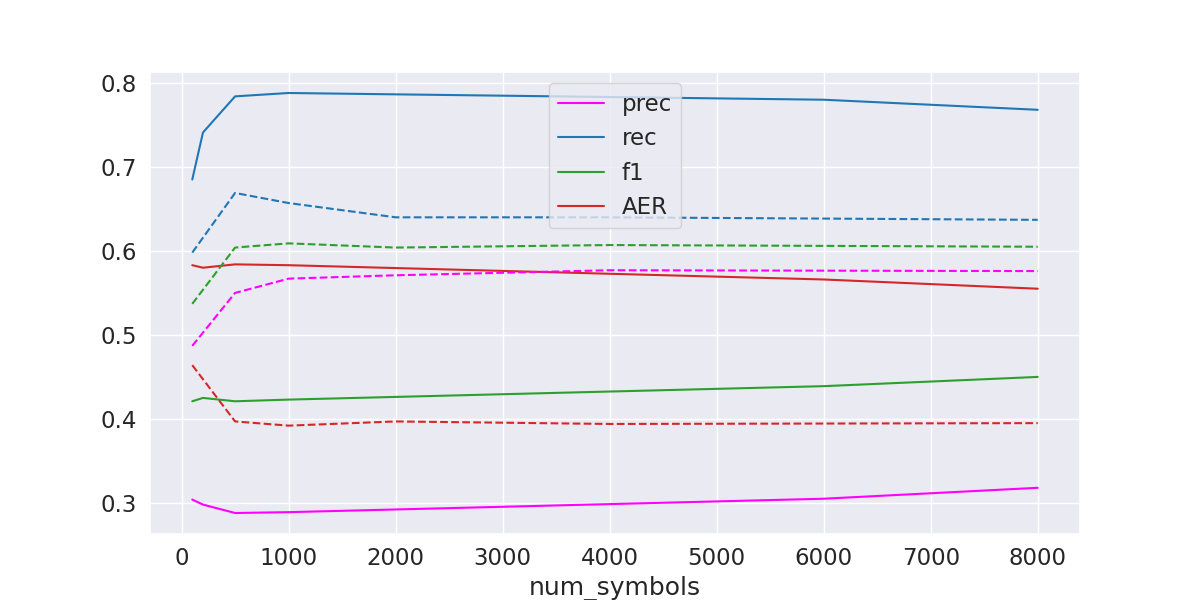
\includegraphics[width=12cm]{../reports/scores_dropout_bpe/space/0.1/union_fastalign.png}
     \caption{Scores for BPE with dropout 0.1, union mode}
 \end{figure}
 
 \begin{figure}[!ht]
     \centering
     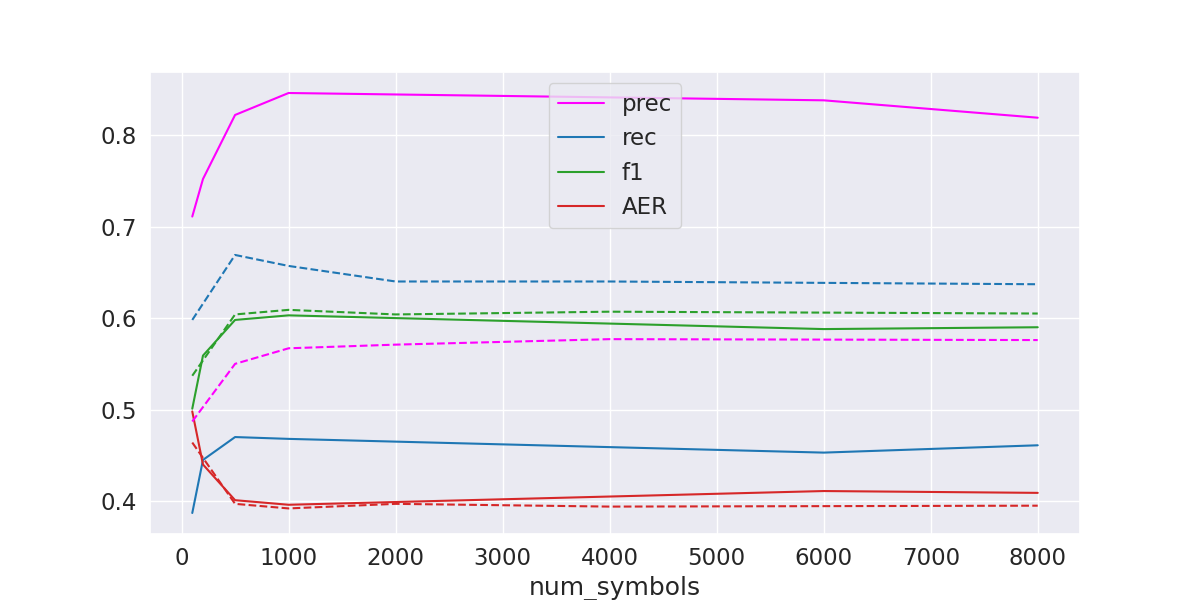
\includegraphics[width=11.5cm]{../reports/scores_dropout_bpe/space/0.1/inter_fastalign.png}
     \caption{Scores for BPE with dropout 0.1, intersection mode}
 \end{figure}

It can be seen that the F1 score improves consistently the more BPE units have been merged. Since there are more merges, there are fewer units, most words are completely merged and the uncertainty of aligning BPE units is lower, since the sentence looks more and more similar to the raw sentence where there are just words. Regarding the threshold case, the following two figures show the scores for threshold 0.3 and 0.7, \textbf{which achieves the best F1 score, namely 0.635}.

\begin{figure}[!ht]
    \centering
    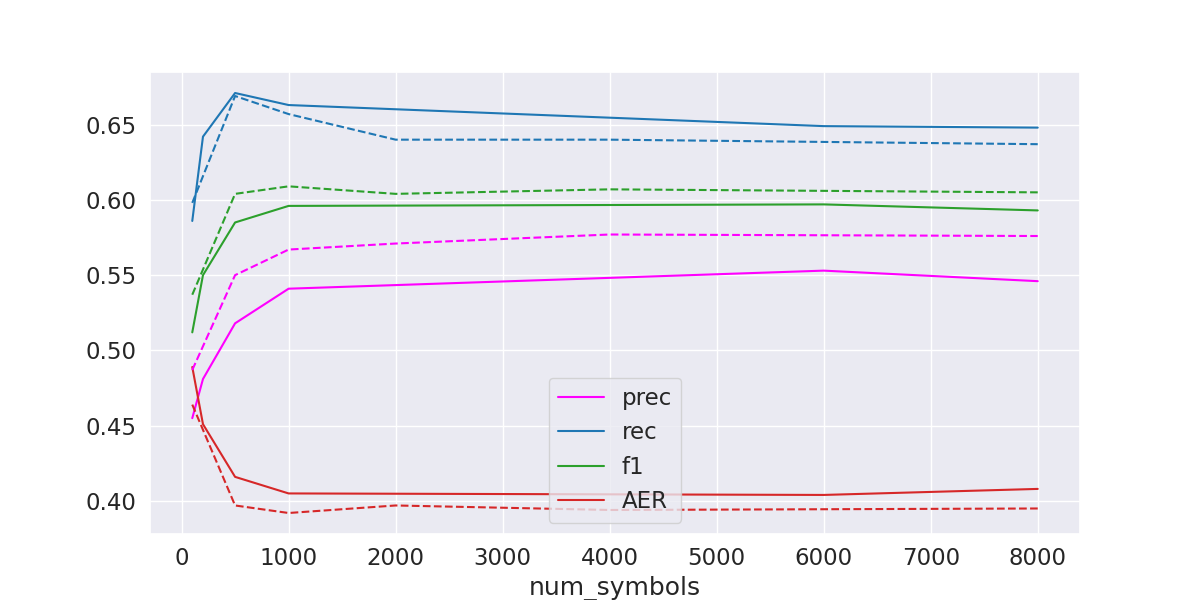
\includegraphics[width=11.5cm]{../reports/scores_dropout_bpe/space/0.1/0.3_thres_fastalign.png}
    \caption{Scores for BPE with dropout 0.1, threshold mode at 0.3}
\end{figure}

\begin{figure}[!ht]
    \centering
    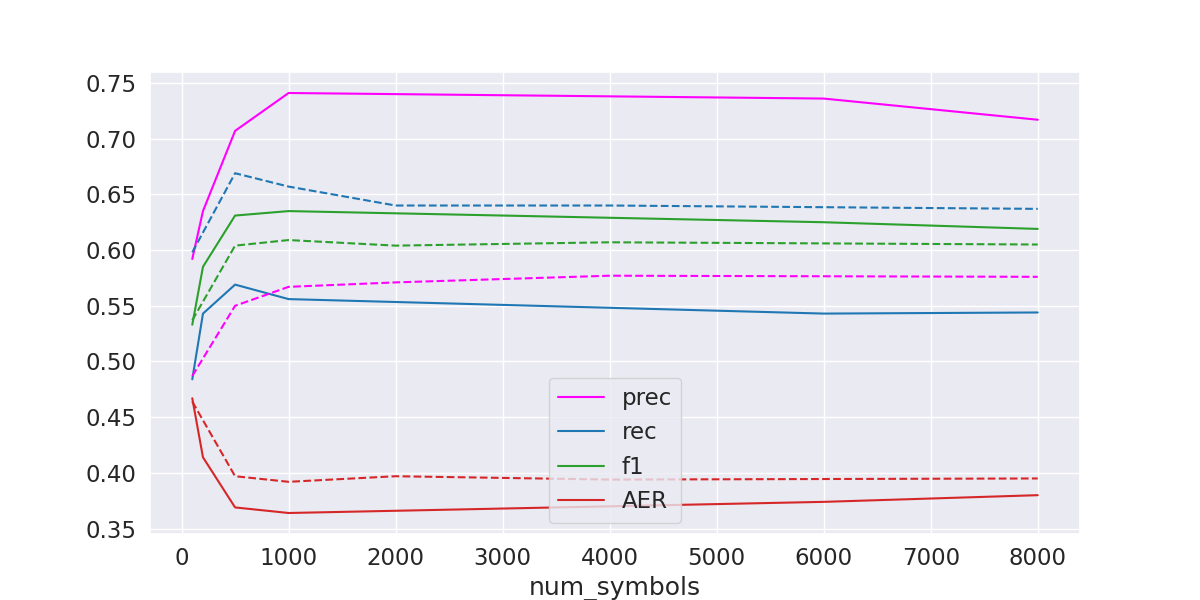
\includegraphics[width=11.5cm]{../reports/scores_dropout_bpe/space/0.1/0.7_thres_fastalign.png}
    \caption{Scores for BPE with dropout 0.1, threshold mode at 0.7}
\end{figure}

It's visible that the scores with the thershold at 0.3 resemble the union case more, and recall goes lower while the precision goes higher for higher threshold values. The optimal result is found at the threshold value of 0.7. This result is replicated when increasing the dropout rate up to 20\% as well as 30\%, and setting the alignment threshold at 0.5. This shows that BPEs are robust to dropout.

In the BPE dropout paper~\cite{provilkov2019bpedropout} the authors only use one dropout percentage, namely 10\% for all languages and 60\% specifically for Chinese and Japanese to match the increase in length of segmented sentences for other languages. The paper hypothesizes that exposing a model to different segmentations might result in better understanding of the whole words as well as their subword units, which is proven by the paper and by this thesis as well. The paper authors also speculate the following:

\begin{quote}
	Results indicate that using BPE-Dropout on the source side is more beneficial than using it on the target side. We speculate it's more important for the model to understand a source sentence, than being exposed to different ways to generate the same target sentence.
\end{quote}

This phenomenon hasn't been the case in this thesis, the results have actually been slightly worse than normal BPE, the difference decreasing the more symbols are employed. A reason for this might be that the corpora are small, or that the languages in the available corpora (English and German) show a different behaviour than the average.

\begin{figure}[!ht]
    \centering
    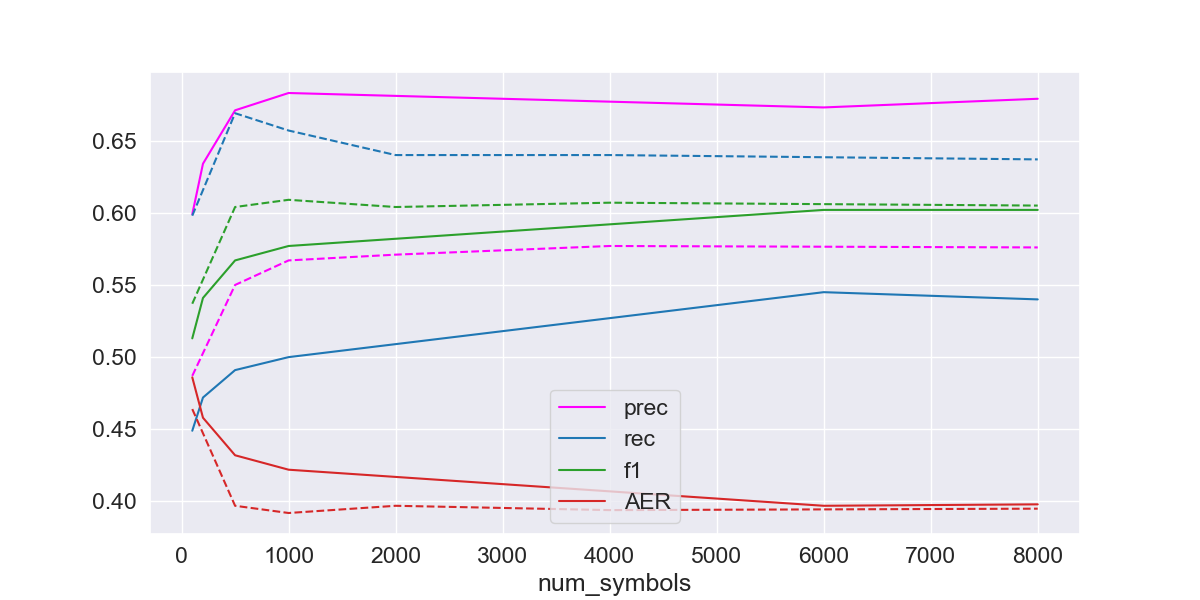
\includegraphics[width=11.5cm]{../reports/scores_dropout_bpe/space/0.1/0.7_thres_fastalign_eng.png}
    \caption{Scores for BPE with dropout 0.1, threshold at 0.7 and BPE only in source language}
\end{figure}

Regarding the improvements of BPE dropout over normal BPE, the authors conclude the following:

\begin{quote}
	The improvement with respect to normal BPE are consistent no matter the vocabulary size. But we see that the effect from using BPE-Dropout vanishes when a corpora size gets bigger.
\end{quote}

This thesis has predominantly been run with a fixed size, relatively small corpus consisting of 10.000 sentences, whereas the paper authors have used much bigger corpora ranging from 133.000 sentences up to 2 million. As a result, the effect of varying corpus size has not been replicated. 

However, it can be seen that for bigger number of merges, the effects of BPE dropout are smaller, since given the bigger number of merges, the segmentations resemble the case where no dropout is applied.

As the BPE dropout paper states, \emph{BPE dropout improves BPE consistently no matter how many merges are performed}. This result is replicated in this paper. Additionally, in the paper they use a fixed dropout rate and they give no information as per the threshold using in determining how to aggregate alignments. \textbf{By experimenting with different dropout and threshold rates, it was possible to improve the F1 score by selecting a dropout rate of 30\%, which is specific to the corpus, in this case English and German, creating 30 segmentations and selecting an alignment threshold of 50\%. This results in a F1 score of 0.685, an improvement of 2\% from the previous case}.

\section{Improvement of the learn BPE algorithm}

When the corpus update algorithm was modified, introducing indexes and frequency counts to reduce iteration, the learn BPE algorithm's runtime was dramatically accelerated. In the beginning, the algorithm starts by creating around 1.5 BPE merges per second. These take a longer time because since they are so frequent, most of the indexes in the corpus are visited and many update operations are done. The less frequent merges are, the faster it is to merge them and update the corpus. The speed of merges per second gets faster and faster until by the time it is finished with the corpus, it is running at roughly 300 merges per second for English and 120 merges per second in German.

After the improvement, the algorithm, on average, needs \textbf{55s to learn BPEs in English, and 1:25min to learn BPEs in German on corpora composed of 10.000 sentences}. The time difference between English and German is due to the fact that there are longer words in German, and therefore, more merge possibilities. In contrast, Sennrich et al.~\cite{sennrich2015neural}'s algorithm needs 2:15min for English and 3:20min for German. The algorithm presented here shows an improvement in speed of 2.5x for English and 2.4x for German. These test have been performed on an Intel Core i5-7200U CPU at 2.5GHz, a 64-bit Windows OS with at 8GB RAM.

A C++ implementation of the BPE algorithm from Sennrich et al. can be found on \href{https://github.com/glample/fastBPE}{Github}, which is capable of learning BPE codes and applying them to a corpus. This package makes use of C++'s advantage to handle memory better than Python, for instance by memory mapping the input file to read it efficiently, and by using multi-threading to pre-compute the BPE splits of all words in the input file. When applied to this thesis' dataset, it barely needs a few seconds to learn BPE codes, making it much faster than the algorithm developed in this thesis. However, this package does not include BPE dropout or any other word separation rather than \emph{</w>} at the end of the word; it is not possible to create BPE tokens without word boundaries using this method. it is assumed that it would not be very complicated to integrate these two aspects into the package, but given that it was created by a PhD student, there are no guarantees of maintenance in the future. In contrast, this thesis' algorithm takes more time but depending on \emph{dropout} and \emph{space} parameters, the algorithm is adapted to both scenarios.

\section{No space results}

Learning BPE units that can handle merges among words takes more time, since there are more possibilities to merge; each end of the word and each beginning of the word can now be merged. In the previous case, there was only a fixed number of merges that could be done inside a word, once the whole word was merged into one unit, no other merges were possible. Now however, that word can be merged with its previous or subsequent tokens.

As with the space case, the algorithm starts at around 0.7 BPE merges per second. While the most frequent merge in the space case is \emph{\_t, h} for English and \emph{e, n} for German, in the no space case the most frequent merges are \emph{e, \_} for English and \emph{e, n} again for German. In the English case, the pair \emph{e, \_} is much more frequent than the pair \emph{\_t, h}, hence it takes more time for this pair to get merged. Afterwards, the number of merges per second increases until plateauing at 40 merges per second, both for English and German. The runtime is \textbf{3:50min for 10.000 merges in English and 4:10min in German}. Since there are more merge possibilities, the algorithm was also run \textbf{for 20.000 merges, with a runtime of 9:30min in English and 10min in German}.

Alignments have been performed without a notion of what words are. Alignments between subword units have been performed as in the previoius cases, but also multiword alignments, which is not the format that Fastalign and Eflomal are prepared to handle. It is therefore expected that the scores will be lower than in the space case, and it is also expected that the more BPE merges are performed, the bigger these segmentations will be, the more words will be merged together, and as a result the more multiword-to-multiword alignments will be present. For instance, the multiword unit \emph{in\_the\_street} might be aligned to \emph{auf\_der\_Strasse}, which would result in the following alignments: \emph{in-auf}, \emph{in-der}, \emph{in-Strasse}, \emph{the-auf}, \emph{the-der} and so on. This brings the precision down dramatically, since most of these alignments are incorrect. For the case of no dropout, the best result for BPE without space separations is a F1 score of 0.477, obtained at 200 symbols, which is a very low number of symbols compared to the previous best scores. The F1 score is also poor relative to the case where merges between words are no allowed.

\begin{figure}[!ht]
    \centering
    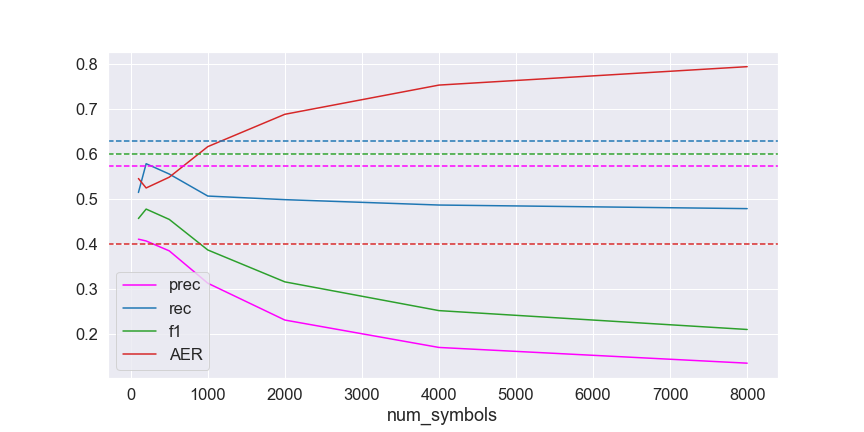
\includegraphics[width=11.5cm]{../reports/scores_normal_bpe/eng_deu_ns_fastalign.png}
    \caption{Scores for no space BPE, no dropout}
\end{figure}

\begin{figure}[!ht]
    \centering
    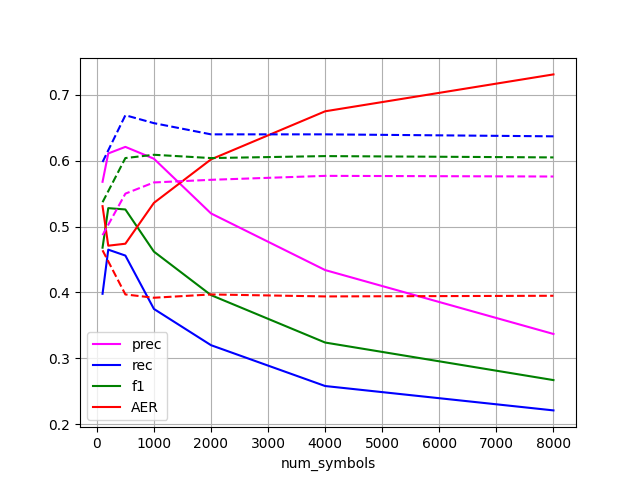
\includegraphics[width=11.5cm]{../reports/scores_dropout_bpe/no space/0.1/scores_ns_0.7_thres.png}
    \caption{Scores for no space BPE with dropout 0.1, threshold at 0.7}
\end{figure}

For the dropout rate of 10\%, results already improve wtih a F1 score of 0.523 for 200 merges and an alignment threshold of 0.7. The maximum F1 score is obtained at a dropout rate of 20\%, with a F1 score of 0.559 for 500 merges and an alignment threshold of 0.5.

\begin{figure}[!ht]
    \centering
    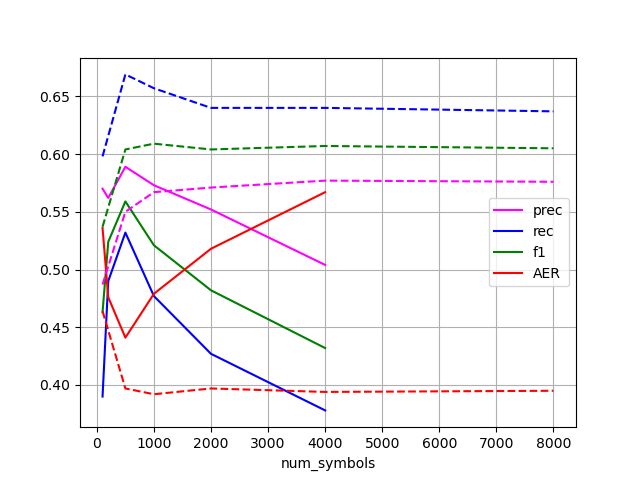
\includegraphics[width=11.5cm]{../reports/scores_dropout_bpe/no space/0.2/scores_ns_0.5_thres.png}
    \caption{Scores for no space BPE with dropout 0.2, threshold at 0.5}
\end{figure}

Experiments with higher dropout rates have also been conducted, namely a dropout rate of 50\% which is very large, half the merges are dropped, with a F1 score of 0.529 for 4000 merges and an alignment tnreshold of 0.3. These parameters are considerably different than the ones previously. The ideal score happens at 4000 merges, which makes sense that it is a bigger number since so many merges are dropped. And the alignment threshold is also very low compared to previous cases, meaning that most alignments are accepted creating a sort of union.

\begin{figure}[!ht]
    \centering
    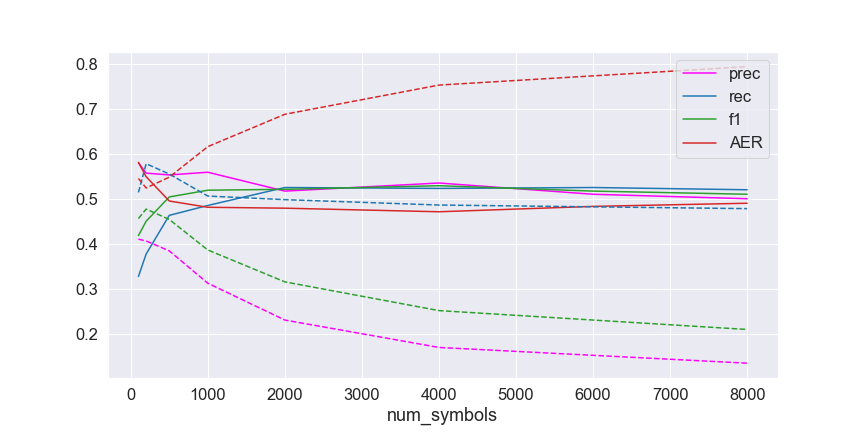
\includegraphics[width=11.5cm]{../reports/scores_dropout_bpe/no space/0.5/scores_ns_0.3_thres.png}
    \caption{Scores for no space BPE with dropout 0.5, threshold at 0.3}
\end{figure}
